\subsection{Problema a resolver}

El siguiente ejercicio se da en el contexto de un museo donde se requiere, por cuestiones de seguridad, colocar sensores de forma tal que todo el piso del museo esté cubierto por los laser que emiten, existen dos tipos de sensores, lo direccionales (que emiten señales horizontales o verticales) y los bidireccionales (que emiten señales hacia ambos lados) y su valor es \$4000 y \$6000 respectivamente. Se pide también que un sensor no este apuntando hacia otro por que esto podria provocar que algún sensor deje de funcionar y no es lo deseado, ademas se pide que en ciertos lugares, definidos como "importantes", haya dos laser pasando simulateamente. El objetivo entonces es encontrar la forma de colocar estos sensores de forma tal que el suelo quede completamente cubierto y que los lugares importantes queden con ambos laser pasando por el y ademas que el costo total de los sensores sea minimo, tambien hay que tener en cuenta que en el museo puede haber paredes que interfieran en los laser de los sensores.

Un ejemplo de este problema es el que está provisto por la catedra


\begin{figure}[H] %[h] Aqui [b] para button [t] para top
	\begin{center}
		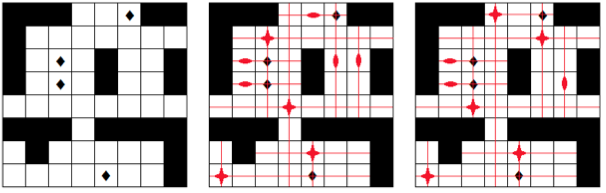
\includegraphics[width=320pt]{../imgs/ej3_ejemploCatedra.png}
	\end{center}
\end{figure}


\subsection{Resolución coloquial}

\subsection{Demostración de correctitud}

\subsection{Complejidad del algoritmo}

\subsection{Código fuente}

\subsection{Instancias posibles}

\subsection{Testing}
